\section{careful prior}

\subsubsection{Example}

\eqn{
U &\sim N(0 , 1)\\
Z &\sim N(2U , 0.09)\\
X &\sim N(0.5Z , 1)\\
Y &\sim N(3U + -Z + 0.5X , 0.25)
}

\begin{figure}[h]
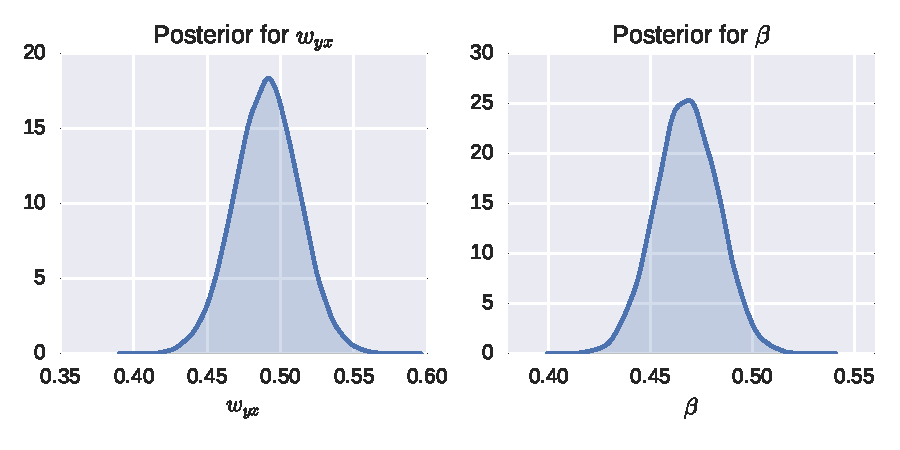
\includegraphics[scale=.3]{prior_no_prior}
\caption{no prior, posterior on $w_{yx}$ centered around $w_{yx}$}
\end{figure}

\begin{figure}[h]
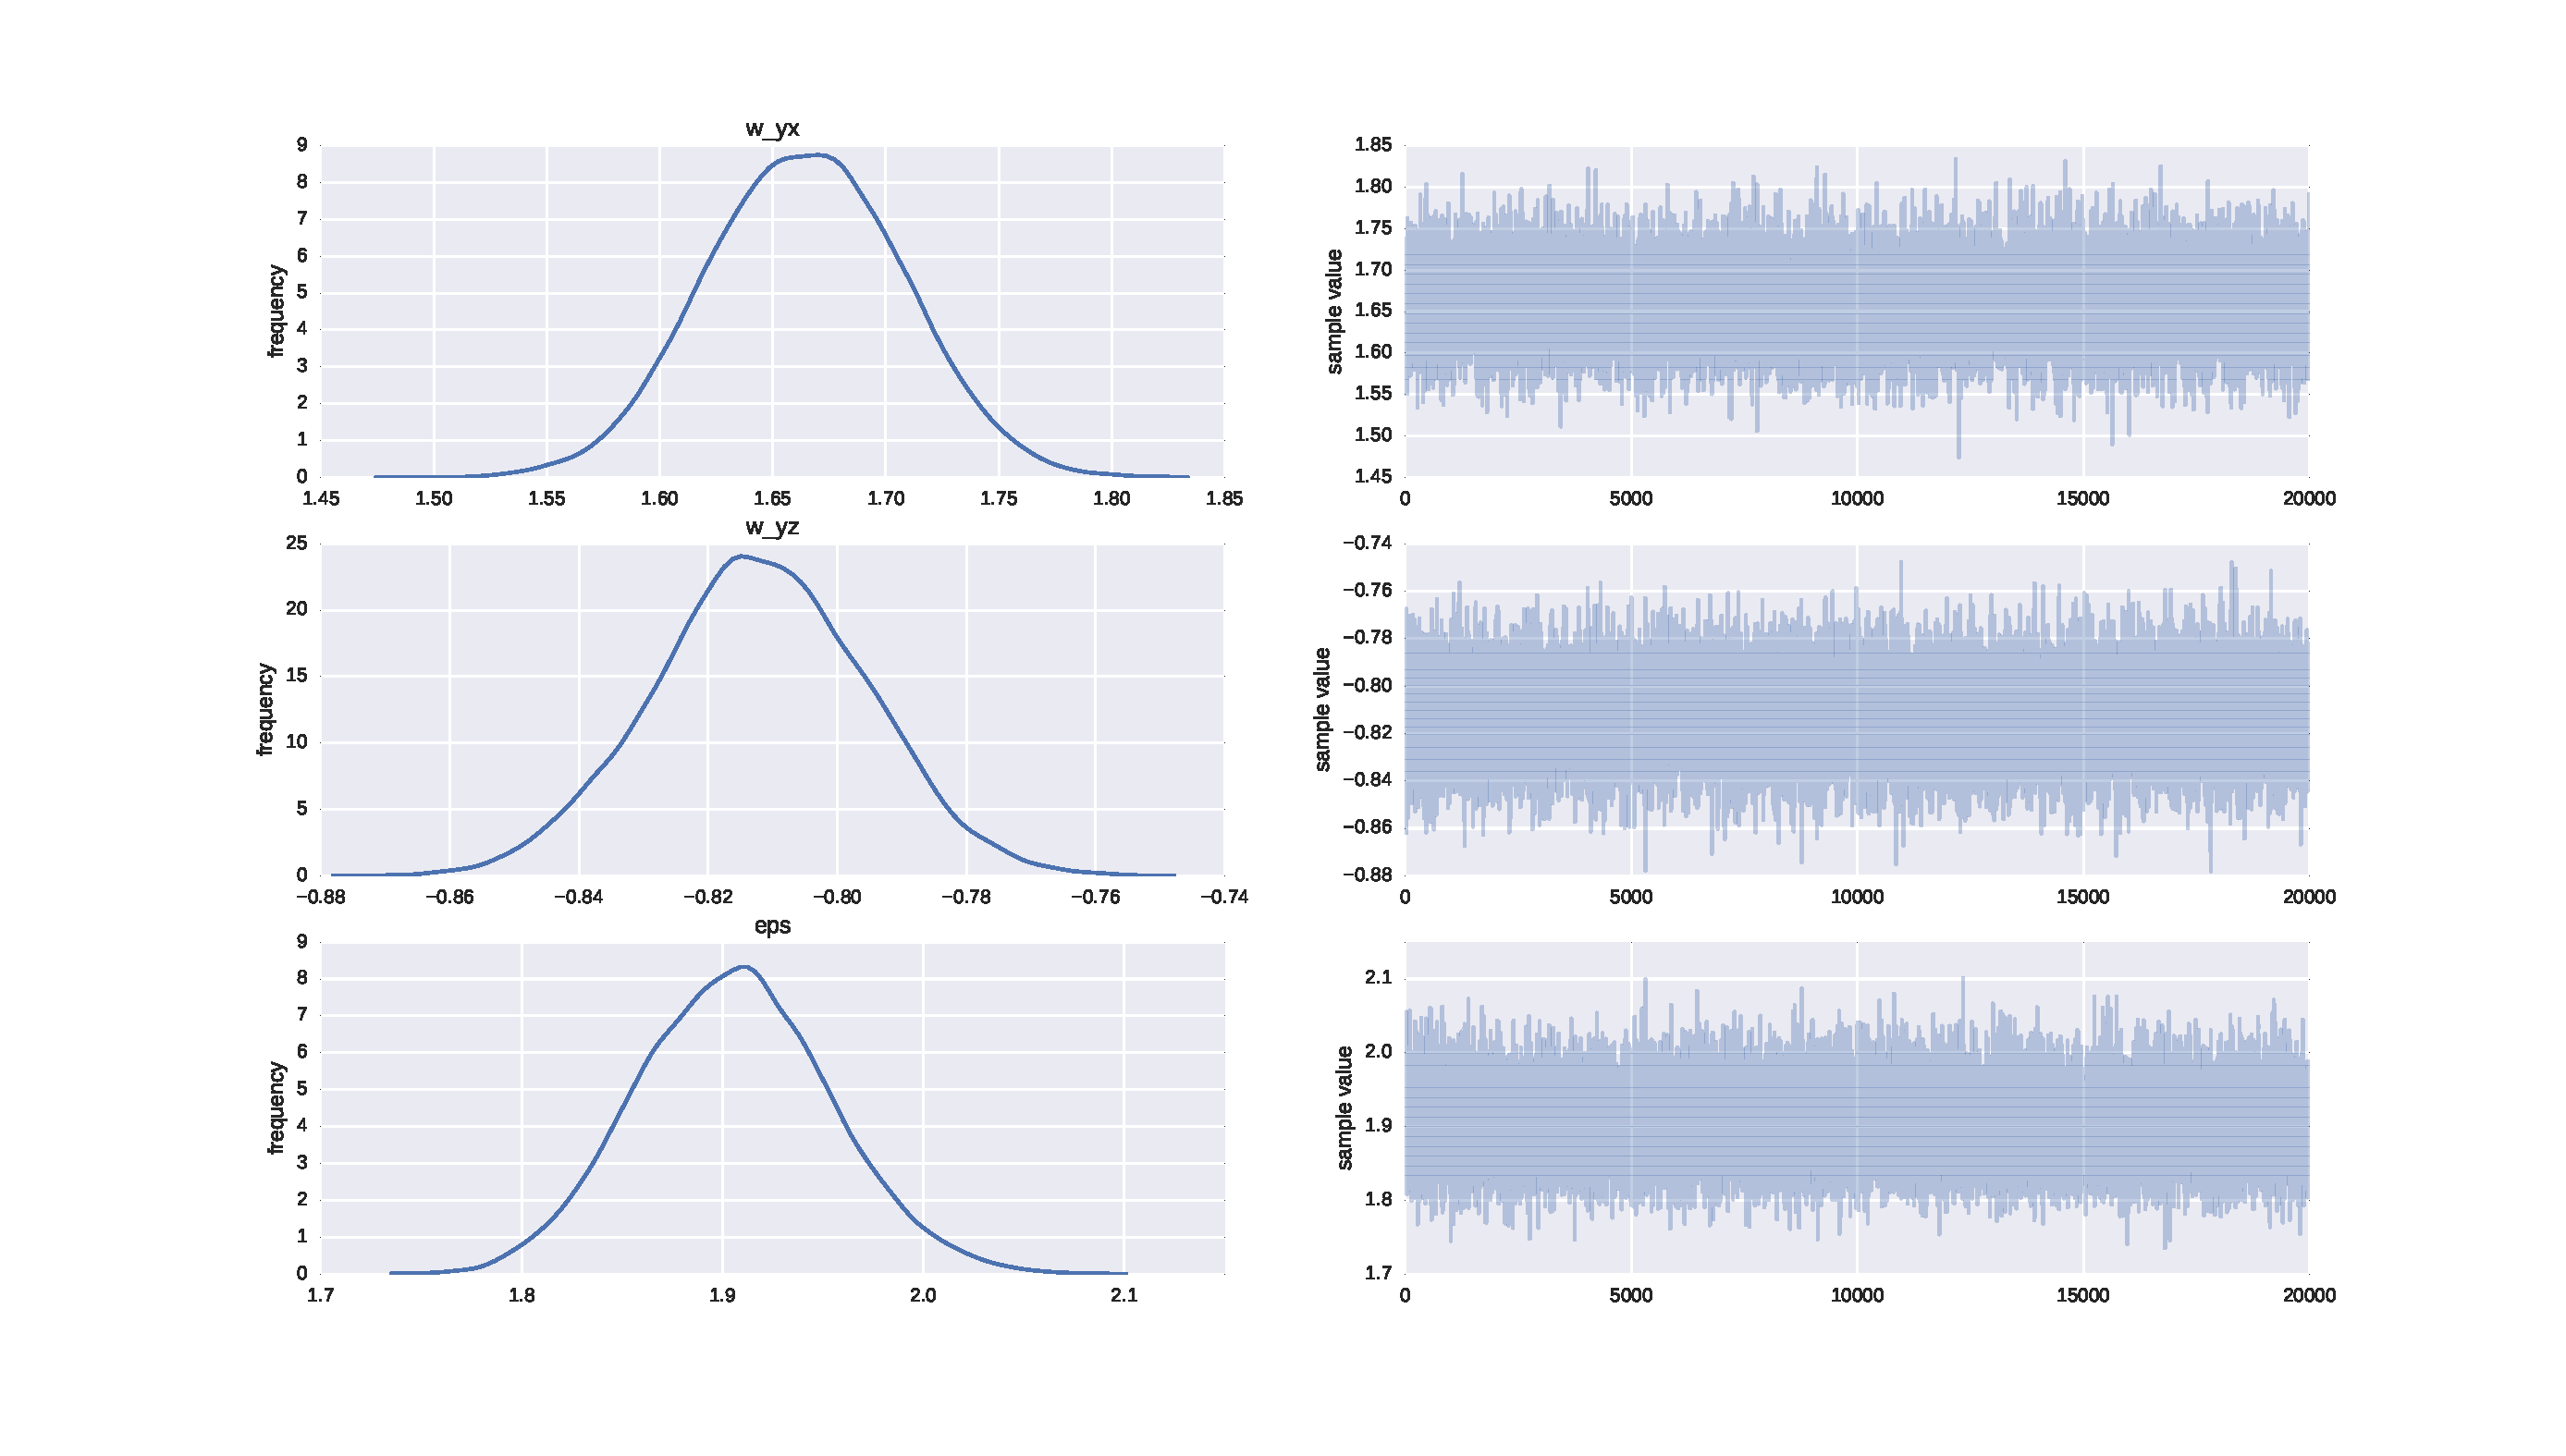
\includegraphics[scale=.3]{prior_bad_prior}
\caption{Prior around $w_{yz}$, $\beta \sim N(w_{yz},\sigma = 0.5)$. The posterior on $w_{yx}$ is biased away from its true value}
\end{figure}



Observational causal inference, the problem of estimating the impact of some intervention in a system from observational data, has been studied in depth, particularly within economics and the social sciences for

The problem of estimating the impact of an intervention in a system from observational data has been studied in depth, particularly in economics and social sciences, for many years. 

They also consider the impact of different assumptions about the relationship between the suggested action $A$ and actual action $X$, which are not captured by structure of the graph.

\section{Causal Discovery}
\label{sec:causal-discovery}

%Cyclic models \citep{Hyttinen2012}

We now move to the much more general problem of learning a causal graph from observational data. In this setting we make much broader assumptions about the structure of the graph. For example, that it is acyclic or that we have no unmeasured confounding variables. We do not assume the existence or directions of any links between the variables. Amazingly, it is possible to infer some aspects of causal structure with such general assumptions. The set of conditional independence in a non-experimental data set indicates some causal structures are more likely than others. In addition, there can be subtle asymmetries in the relationship between the joint distribution of cause and effect and the distributions of cause given effect and effect given cause. These clues are the key to causal discovery algorithms.

%There is also work on inferring causal structure from experiential data \ref{}. We discuss this further in section XXX.

Causal discovery is a much grander goal than causal effect estimation given a known causal network. Arguably, if achieved, it would equate to the automation of scientific discovery. We need simply supply our algorithm with a vast collection of variables (regardless of their relevance to the problem) and it would learn the causal structure and from that allow us to estimate the effects of any intervention we cared to make. Unfortunately, causal discovery is very hard. Even with the assumption that the causal graph is acyclic and there are no latent variables, the number of possible graphs grows exponentially with the square of the number of variables .

% - some intuition here about the strength of the signal we get from causal discovery. Small initial errors in greedy approaches can cascade leading to unstable inference and large losses \ref{sprites?}. Talk about the numerical as well as the statistical issues here. 

In the next sections we briefly survey the key approaches to causal discovery. We roughly divide the methods into those based on those that exploit the connection between the conditional independencies in a joint distribution and the structure of a causal model and those that leverage assumptions about the functional form of the relationships between cause and effect. 

%This is not the only way we could have grouped them. There is also a separation between constraint based algorithms, that XXXX and those that search and score multiple graph structures before selecting the best. There are also hybrid methods \ref{}  

\subsection{Conditional independence based methods}
One general approach is to look for clues about the structure of the network in the conditional independence relations in the distribution. For any Bayesian network, $G$, (causal or not) we can read of conditional independencies in the joint distribution from the structure of the network. If a set of variables $Z$ d-separates $X$ and $Y$ in $G$ then $(X \ci Y|Z)$ in the distribution $P$. However, we want to work in the other direction, from conditional independence in the distribution to the structure of the network. This requires that we assume the reverse condition: $(X \ci Y|Z)$ in $P$ must imply $Z$ d-separates $X$ and $Y$ in $G$. This assumption, commonly referred to as  \textbf{\textit{faithfulness}} \ref{Sprites2000}, says there are no additional independence relations that are satisfied in $P$ but not in all distributions $\boldsymbol{P'}$ that are compatible with $G$. Stating that $P$ is faithful to $G$ is equivalent to $G$ is a \textbf{\textit{perfect map}} \citep{pearl1988probabilistic} for $P$.

Faithfulness is an assumption. It does not always hold and we cannot verify it from the observational data we wish to use for causal inference. However, most distributions generated by a causal Bayesian network will be faithful to that network. For faithfulness to be violated, different causal effects must exactly balance one-another out. For example, consider a simple binary variable model of chocolate consumption, income and obesity (figure). If the coefficients in the conditional probability tables are just right then the direct effect of chocolate on obesity will exactly balance the indirect effect through income and obesity will appear independent of chocolate consumption. However, this independence is not stable. It would disappear under a small perturbation to any of the parameters. In discrete systems, violations correspond to the solutions to polynomial equations over values in the CPD tables and thus are a space of measure zero with respect to all possible distributions associated with the graph \citep{Koller2009}. 

Given the faithfulness assumption, our causal discovery problem reduces to finding the set of Bayesian networks that have exactly the dependency structure as we observe in $P$. This set can also be referred to as the Markov equivalence class compatible with $P$.

\subsubsection{Without hidden common causes}
The strong assumption that there are no hidden variables that cause two or more variables in $\boldsymbol{V}$ significantly reduces the 'search space' of Bayesian networks we must consider. This assumption is referred to as causal sufficiency \citep{Sprites2000}.

We will begin with a brute force algorithm (described as the SGS algorithm in \citet{Sprites2000} and IC algorithm in \citet{Pearl2000}). While it is impractical for all but the smallest of networks, it demonstrates key concepts that also underlie the more useful and complex algorithms we will discuss later. 

\begin{table}[H]
 \begin{tabularx}{\textwidth}{X}
 \hline
\rule{0pt}{2.5ex} 
 \textbf{The SGS (or IC) Algorithm}\\
 \hline
 \rule{0pt}{2.5ex}
\textbf{Input:} A distribution $P$, over variables $\boldsymbol{V}$, that was generated by and is faithful to an (unknown) Bayesian network $G$\\
\textbf{Output:} A partially directed network that represents the Markov equivalence class of $G$\\
 \begin{enumerate}[itemsep=8pt]
  \item Join all pairs of vertices $(a,b) \in \boldsymbol{V}$ with an un-directed link to form a complete graph.
  \item For each link $a-b$ search for a set $\boldsymbol{S}_{a,b} \subseteq V \setminus \{a,b\}$ that renders $a$ and $b$ conditionally independent. If such a set (including the empty set) exists then $a$ and $b$ cannot be directly connected in $G$ so delete the link.
  \label{alg:SGSexponential}
  
  \item For all pairs of non-linked variables $(\alpha,\beta)$ with a common neighbour, $c$, if $c \notin \boldsymbol{S}_{\alpha,\beta}$, then $c$ must be a collider in the path $\alpha,c,\beta$ so  add arrows to direct the links $\alpha-c$ and $\beta-c$ towards $c$.
  \label{alg:SGScolliders}  
  \item Recursively try to orient any edges that remain un-directed to avoid creating cycles (because they are not there by assumption) and additional colliders (because any colliders were found in step \ref{alg:SGScolliders}).
  \label{alg:SGSfinal}
\end{enumerate}\\
 \hline
\end{tabularx}
\end{table}

The SGS algorithm utilises the fact that a collider structure (figure \ref{fig:dseptripple4}) induces a distinct conditional independence relation. Assuming you have a consistent conditional independence test, it converges to return a partially directed network that represents the Markov equivalence class for the generating causal model. Unfortunately the number of conditional independence tests required for step \ref{alg:SGSexponential} grows exponentially (in the worst case) with the number of variables. Not only that, but for each edge that is in the true network, the algorithm will always tests all other possible subsets of variables. If the assumption that there are no hidden common causes or that the distribution is faithful are violated, step \ref{alg:SGScolliders} of the SGS algorithm can produce double headed arrows.

The PC algorithm \citet{Sprites2000} modifies step \ref{alg:SGSexponential} of the SGS algorithm to utilise the fact that if two variables $(a,b)$ are conditionally independent given some set, they will also be conditionally independent given a set that contains only variables adjacent to $a$ or $b$. It also checks for low order conditional independence relations before higher order ones. This allows it to exploit any sparsity in the true network, leading to much better average case performance  \citep{Sprites2000} (although the worst case, where the true network is complete, is still exponential). With finite data, the order in which the links are considered can change the output (unlike for SGS). The effect of wrongly removing a link early on flows through to later conditional independence tests by changing which nodes are considered adjacent.

\begin{table}[H]
 \begin{tabularx}{\textwidth}{X}
 \hline
\rule{0pt}{2.5ex} 
 \textbf{The PC Algorithm}\\
 \hline
 \rule{0pt}{2.5ex}
\textbf{Input:} A distribution $P$, over variables $\boldsymbol{V} = \{V_{1}...V_{k}\}$, that was generated by and is faithful to an (unknown) Bayesian network $G$\\
\textbf{Output:} A partially directed network that represents the Markov equivalence class of $G$\\
 \begin{enumerate}[itemsep=8pt]
  \item As for SGS
  \item \textbf{for} each link $a-b$:
  \begin{itemize}[label={}]
   \item $n = 0$
   \item $\boldsymbol{A}_{a,b} = \{A_{1}...A_{j}\}$ be the set of nodes adjacent to $a$ and/or $b$
   \item \textbf{while} $a$ and $b$ are connected and $n < j$:
   \item 
    	\begin{itemize}[label={}]
    	\item \textbf{if} any subset of size $n$ of $\boldsymbol{A}$ makes $a$ and $b$ conditionally independent:
    	\item \begin{itemize}[label={}]
    			delete the link
    		  \end{itemize}
    	
    	\item $n = n+1$
    	\end{itemize}
  \end{itemize}   
  \item as for SGS
  \item as for SGS
\end{enumerate}\\
 \hline
\end{tabularx}
\end{table}

The PC algorithm also returns a set of Markov equivalent networks consistent with the distribution. Since we have assumed there are no hidden variables, for any single graph in this set we can calculate causal effects from the truncated product formula \ref{eq:truncatedproduct}. We can then bound the true causal effect by combining the results for the all the networks. This procedure is the IDA algorithm \citep{Maathuis2009} and has been found to outperform standard regularisation techniques at finding causal effects in a high-dimensional yeast gene expression data set \citep{Maathuis2010}. An implementation is available in the R package \citep{Kalisch2012} 

\subsubsection{With hidden variables}
There are an number of difficulties in extending the approach of the last section to deal with the case where there are latent variables. With an unknown number of hidden variables there are infinity many possible structures to search over. In addition, the space of causal networks is not closed under marginalisation. If we have a distribution that $P'(\boldsymbol{O},\boldsymbol{U})$ generated by and is faithful to a network $G$ the distribution $P(\boldsymbol{O})$, that results from marginalising over $\boldsymbol{U}$, may not be faithful to any Bayesian network (see figure \ref{fig:DAGSnotclosed}). The key to constraining the space of possible models is that many latent structures are equivalent (under transforms of the hidden variables).

\begin{figure}
\centering
 \begin{tikzpicture}[->,>=stealth',shorten >=1pt,auto,node distance=1cm,  thick,main node/.style={observed},lt/.style={latent}]
 %nodes
\node[lt](1){U}; 
\node[main node, below left = of 1](2){B};
\node[main node, below right = of 1](3){C};
\node[main node, above left= of 2](4){A};
\node[main node, above right = of 3](5){D};

 \path[every node/.style={font=\sffamily\small}]
    (1) edge node {} (2)
    	edge node {} (3)
    (4) edge node {} (2)
    (5) edge node {} (3);
    	
\end{tikzpicture}
\caption{A distribution faithful to this DAG is not faithful to any DAG over the variables $\{A,B,C,D\}$ after marginalising over $U$. }
\label{fig:DAGSnotclosed}
\end{figure}
 
\begin{theorem}
\citet{Verma1993} For every latent structure there is a dependency equivalent structure such that every latent (unobserved) variable is a root node with exactly two children .
\end{theorem}

Since we only care about the causal relationships between observed variables, it is sufficient to search over networks where any hidden variables have no parents and directly cause two of the observed variables. Instead of representing hidden variables explicitly we can capture the necessary independence relations with a more general graphical model that supports bi-directed edges that play the role of a hidden confounding variable. These models, referred to as maximal ancestral graphs (MAGs) are closed under marginalisation and conditioning. 

For any DAG with latent (and selection) variables there is a unique MAG \citep{Richardson2002}. This makes it possible to extend the PC algorithm to latent structures, resulting in the FCI algorithm \citep{Sprites2000}. The logic behind the algorithm is very similar. Certain structures are ruled out as a consequence of being inconstant with the observed conditional independence relations. The output is an equivalence class of MAGs, which can be represented graphically as a partial ancestral graph PAG \citep{Spirtes1995}. Assuming there are no selection variables, the PAG can contain four types of link:

\begin{enumerate}
\item $X \rightarrow Y$, meaning $X$ causes $Y$
\item $X \leftrightarrow Y$, meaning there is a latent variable that causes $X$ and $Y$.
\item $X\ {\circ} {\rightarrow}\ Y$, either $X$ causes $Y$ or a latent variable causes both.
\item $X\ {\circ} {-}  {\circ}\ Y$, either $X$ causes $Y$ or $Y$ causes $X$ or a latent variable causes both.
\end{enumerate}

The circles indicate where it is ambiguous if there should be an arrowhead (IE where there is one in some MAGs and not in others in the equivalence class). Counter-intuitively it is sometimes possible to  rule out or confirm the existence of a confounding variable and fully determine the causal type of a link (see examples in figure \ref{fig:FCIExamples}). 


\begin{figure}
\centering
 \begin{subfigure}[t]{0.4\textwidth}
 \centering
 \caption{True DAG}
 \begin{tikzpicture}[->,>=stealth',shorten >=1pt,auto,node distance=.7cm,  thick,main node/.style={observed},lt/.style={latent}]
 %nodes
\node[lt](1){U}; 
\node[main node, below left = of 1](2){B};
\node[main node, below right = of 1](3){C};
\node[main node, above left= of 2](4){A};
\node[main node, above right = of 3](5){D};

 \path[every node/.style={font=\sffamily\small}]
    (1) edge node {} (2)
    	edge node {} (3)
    (4) edge node {} (2)
    (5) edge node {} (3);
    	
\end{tikzpicture}
 \end{subfigure}
 \begin{subfigure}[t]{0.4\textwidth}
  \centering
  \caption{Partial ancestral graph}
 \begin{tikzpicture}[->,>=stealth',shorten >=1pt,auto,node distance=.7cm,  thick,main node/.style={observed}]
 %nodes

\node[main node](1){A};
\node[main node, below right=of 1](2){B};
\node[main node, right=of 2](3){C};
\node[main node, above right=of 3](4){D};

 \path[every node/.style={font=\sffamily\small}]
    (1) edge[pil] node {} (2)
    (2) edge node {} (3)
    (3) edge node {} (2)
    (4) edge [pil] node {} (3);    	
\end{tikzpicture}
\end{subfigure}
\par\bigskip 
 \begin{subfigure}[t]{0.4\textwidth}
 \centering
 \caption{True DAG}
 \begin{tikzpicture}[->,>=stealth',shorten >=1pt,auto,node distance=0.7cm, thick,main node/.style={observed},lt/.style={latent}]
 %nodes

\node[main node](1){C};
\node[main node, above left=of 1](2){A};
\node[main node, above right=of 1](3){B};
\node[main node, below=of 1](4){D};

 \path[every node/.style={font=\sffamily\small}]
    (1) edge node {} (4)
    (2) edge node {} (1)
    (3) edge node {} (1);    	
\end{tikzpicture}
\end{subfigure}
 \begin{subfigure}[t]{0.4\textwidth}
  \centering
  \caption{Partial ancestral graph}
 \begin{tikzpicture}[->,>=stealth',shorten >=1pt,auto,node distance=0.7cm,  thick,main node/.style={observed}]
 %nodes

\node[main node](1){C};
\node[main node, above left=of 1](2){A};
\node[main node, above right=of 1](3){B};
\node[main node, below=of 1](4){D};

 \path[every node/.style={font=\sffamily\small}]
 	(1) edge node {} (4)
    (2) edge [pil] node {} (1)
    (3) edge [pil] node {} (1);    	
\end{tikzpicture}
\end{subfigure}
\caption{FCI examples: true graph and FCI output}
\label{fig:FCIExamples}
\end{figure} 

The FCI algorithm can be made complete such that it discovers all aspects of the true causal structure that are identifiable from the conditional independence relations of a distribution over observed variables and the faithfulness assumption \citep{Zhang2008}. More recently \citet{Colombo2012} have proposed the RFCI algorithm, which in some cases returns more ambiguous links than FCI but is substantially faster. \citet{Claassen2013} point out that the problem of learning sparse causal networks from data is not NP-hard and propose the FCI+ algorithm, that requires $O(N^{2(k+2)})$ conditional independence tests, where $k$ is the maximum node degree over the observed variables. 

Latent variables can create constraints on the marginal distribution over the observed variables that cannot be expressed in term of conditional independencies. These generalised constraints can be expressed and leveraged within nested Markov models \citep{Richardson2012,Shipster2014} 


%\renewcommand{\arraystretch}{1.5}
%\begin{tabular}{| c | c | p{4cm} | c | c | c |}
%\hline
%  \textbf {Alg.} &\textbf{ Method }& \textbf{Scales (num.vars) }& $\sim $ \textbf {Vars} & \textbf {Latent } & \textbf {Reference} \\
%  \hline
%  IC/SGS & Constraint based & Exponential & 10 & No & Pearl(2000)/Sprites(2000)\\
%  \hline
%  PC & Constraint based & Worst case exponential, polynomial for sparse graphs & 5000 & No & Sprites(2000) \\ 
%  \hline
%  FCI & Constraint based & Worst case exponential, polynomial variant FCI+ for sparse graphs & 30 & Yes & Sprites(2000) \\
%  \hline
%  RFCI & Constraint based & ? & 500 & Yes & Colombo(2012) \\
%  \hline
%  GES & Search \& Score  & Worst case exponential & 50 & No & Chickering(2002) \\
%  \hline
%  MMHC & Hybrid & ? & 5000 & No & Tsamardinos(2006) \\
% \hline
%\end{tabular}

All the algorithms discussed in this section rely on being able to perform conditional independence tests. This is non-trivial with high dimensional data. If the functional relationship between the variables is linear with Gaussian noise then the network represents a multivariate normal distribution and a pair of variables are conditionally independent if and only if the corresponding entry in the inverse correlation matrix is non-zero \citep{Koller2009}. Where the functions are non-linear one can apply kernelised independence tests \citep{Gretton2008,Zhang2012}


\subsection{Discovery with functional models}
The algorithms we have considered so far return a Markov equivalence class. They cannot distinguish between two models that result in the same set of conditional independence relations. Consider the very simple case where  there are only two variables and the possible causal structures are $X \rightarrow Y$ or $Y \rightarrow X$. These models have the same dependency structure but in one case $P(Y|do(X)) = P(Y|X)$ and in the other $P(Y|do(X)) = P(Y)$. No algorithm relying purely on conditional independence relations can separate these two cases. 

Let us focus only on the two variable case $X \rightarrow Y$ or $Y \rightarrow X$. What possible clues could there be in the distribution $P(X,Y)$ that could indicate which causal model it was generated from? Recall the functional definition of causality (section \ref{sec:SEM}). There are a number of assumptions about the form of the functions that can allow us to identify the causal direction: non-invertable functions, additive noise \citep{Hoyer2009}, post-non-linear additive noise \citep{Zhang2008a} or linear models with non-Gaussian noise \citep{Hoyer2012}.

The causal direction can also be identified via a connection between casual discovery and semi-supervised learning \citep{Janzing2012}. Suppose we are trying to learn $\P{Y|X}$. The goal of semi-supervised learning is to improve our estimate of $\P{Y|X}$ by leveraging additional data sampled from $\P{X}$. However, if the true causal model is $X \rightarrow Y$ then their is some function mapping values of $X$ to $Y$ which should be invariant to any changes in the input distribution $\P{X}$. Therefor $\P{X}$ should be independent of $\P{Y|X}$ and semi-supervised learning should not perform any better than standard supervised learning. However if the true causal model is $Y \rightarrow X$ then variations in the $\P{X}$ can result from both the input distribution over $Y$ and the mapping from $X$ to $Y$ and semi-supervised learning could help. This assumption of independence of mechanism and input can also allow the identification of the causal direction in SEMs even where the functions are deterministic and invertable \citep{Daniusis2010}. \citet{Janzing2012a} leverage an information geometric viewpoint of the independence of mechanism and input to infer the causal direction between a pair of associated variables.  

Instead of positing a functional restriction on the relationship between variables and then developing theory to exploit that assumption, \citep{LopezPaz2014} propose learning what the causal relationship looks like from data. They assume there will be a difference between the relationship of $\P{X}$, $\P{Y}$ and $\P{X|Y}$ between $X \rightarrow Y$ versus $Y \rightarrow X$. Their algorithm requires a data set in which each row is itself a data set consisting of pairs of variables $(x_i,y_i)$ with a label indicating the direction of causality between $X$ and $Y$. They use a kernel mean embedding to represent the distributions $\P{X}$, $\P{Y}$ and $\P{X|Y}$ as features for each individual sub-data set and train an algorithm to learn the direction of causality. Unfortunately we do not have a large collection of data sets where the causal direction is known to train such a model. \citet{LopezPaz2014} instead use a simulated data set so their model will necessarily be based on the assumptions they make when generating the data. Nonetheless this approach makes it possible to rapidly construct a model from a wide range of possible assumptions, without doing a lot of theory to design a specific algorithm optimised to that setting. 

\citep{Peters2014} have extended results from the bi-variate case to the multivariate setting. They show that if we can come up with a condition that guarantees identifiability for the bi-variate case, we can extend that result to get the conditions under which the multivariate case is identifiable. They build on this to develop an algorithm that allows the construction of causal graphs based on the additive noise assumption. 

\chapter{More stuff}
%\chapter{List of software programs for causal inference}

\begin{itemize}
\item Pcalg. A library in R that implements ...
\item Tetrad.
\item There has to be a library for the Bayesian trees thing
\item Linear regression (you can do this anywhere)

\end{itemize}


Notorious paper Automated Inferences of Criminality using Face Images. - What possible actions could we take? Ban people with most risky 'face types' from critical jobs? But dependent on causal structure, conditioning on the fact that people are in a position to apply for such jobs could reverse the dependency. Ones facial appearance is a readily observable characteristic and there is evidence that people implicitly make assumptions on the basis of it. Consider trials where people with 'more criminal' faces got longer sentences for similar crimes. 
%\chapter{Causality \& Interpretability}

%\chapter{Causality \& Fairness}

Generalisation error weights towards regions where density of x is high (it does not care about minorities). 

As machine learning is incorporated into decision making systems that have fundamental impacts on people’s lives, such as in employment, criminal justice, health and financial services, there are increasing concerns over transparency and fairness \citep{WMD, etc}. Realisation that machine learning algorithms can be inherit biases from the data we feed into them and the choices those building them make about what variables to include, etc. 

The European Union’s General Data Protection Regulation \citep{Goodman2016}\todo{check}, due to come into effect in 2018, requires that people can obtain "meaningful information about the logic involved" in an automated decision process . It also stipulates that such decisions should not be based on special categories of personal data (related to ethnicity, political and religions affiliation or sexuality) unless there "suitable measures" to safeguard individual interests. A key concern is discrimination against disadvantaged groups. 

Discrimination is frequently defined in terms of either disparate treatment- treating otherwise similar individuals differently on the basis of a protected attribute such as race or gender, or disparate impact - a process that yields a significant difference in outcome between groups. We consider how the notions of disparate treatment and impact may be formalised and the implications of how this is done for machine learning. We examine the overlap between the motivations for interpretable and causal models, especially with respect to assessing fairness. We look at how causal models mitigate some of the trade-offs between transparency and predictive accuracy and we examine to what extent the causal relationship between an attribute, any protected attributes and the outcome of interest is relevant to assessing the impact on fairness of its inclusion in a machine learning model.

The lack of part-time work in tech could be argued to constitute indirect discrimination against women. 
A fear that advertising themselves as supporting flexible working options would attract candidates who lacked drive and ambition.
Cultural bias that favours those driven by monetary ambition against those 


Stability - a non causal model can't tell us about a simple do type operation on  a single variable. 

More broadly, we could draw a model representing the system now that could tell us the result of an intervention on a particular variable (such as setting gender), but the system itself could change (for example with customer preferences). There is a notion that a true causal model should be invariant for all time.

Connection to Simpson's paradox. But what should we condition on? \citep{Romie2010} argue that looking at the department level is the correct viewpoint, since this the point at which hiring decisions were made. However, it could be argued that if one department was attracting a large number of higher quality candidates, the overall size of that department should be higher and that the results seen at Berkeley reflected a bias in favour of male dominated fields. 

Different measures of discrimination - is there a difference between groups (after conditioning on xxx)

To understand how we measure and penalise discrimination, we need to take a step back and ask what are the underlying motivations for fairness?

These differences in underlying cause suggest differences in the approach we should take to remedy them.  

%\section{How does discrimination arise in ML models}
\begin{itemize}
\item bias in historical decisions fed in as training data
\item selection bias in input data, due to deliberate or implicit discrimination such as stop and search
\item deliberate manipulation on the part of the person building the model.
\item The hardest case is historical disadvantage, creating genuine differences between relevant attributes of groups.
\item in bias in the label - what happens if you hire minorities but then your staff treat them badly and as a result they under-perform or leave.  
\end{itemize}

%\section{Defining Descrimination}

Define discrimination in terms of causal effect of protected variable in decision making process. 

\citep{Romei2012} note the relevance of causal inference on discrimination analysis.

“the central question in any employment- discrimination case is whether the employer would have taken the same action had the employee been of 7A recurring problem known as the omitted-variable bias.
A multidisciplinary survey on discrimination analysis 9
a different race (age, sex, religion, national origin etc.) and everything else had been the same” (Carson v. Bethlehem)


Let us mathematically define disparate treatment and disparate impact with respect to a statistical model. We will focus on discrete variables for notational simplicity. Assume we have an outcome of interest $Y$, protected attributes $X$, other covariates $Z$ and a (potentially stochastic) model $f$ that maps $\{x, z\}$ to $y_f \in Y$. For a given model $f$, we have a distribution over the predicted outputs given the inputs, $\P{Y_f|X,Z}$
\vspace{.2cm}
\begin{definition}{Disparate Impact}: A model, $f$, that produces a predictive distribution $\P{Y_f|X,Z}$ has disparate impact if the marginal distribution over the predicted outcome, $Y_f$, depends on a protected attribute.
\eqn{
\exists \set{x_1,x_2} \subset X: \sum_z{\P{Y_f|Z,x_1}\P{Z|x_1}} \neq \sum_z{\P{Y_f|Z,x_2}\P{Z|x_2}}
}
\end{definition}

\begin{definition}{Disparate Treatment}: A model yields disparate treatment if people with identical attributes (excluding protected attributes) are treated differently. 
\eqn{
\P{Y_f|Z,X} \neq \P{Y_f|Z}
}
\end{definition}

Avoiding treating people differently purely on the basis of attributes such as ethnicity and gender and avoiding large differences in important outcomes such as education and income between such groupings both seem like desirable goals. Unfortunately, in general, they conflict with one another, see theorem \ref{thm:disparate_conflict}. Any variable we might wish to avoid discriminating on will be correlated to some other measurable covariate $Z$, making it impossible to avoid both disparate treatment and disparate impact. 
\vspace{.2cm}
\begin{theorem} 
\label{thm:disparate_conflict}
Disparate impact and disparate treatment conflict. Given covariates $Z$ and protected attributes $X$, a model, $f$, cannot be fair with respect to both disparate impact and disparate treatment unless $\P{Z|X} = \P{Z}$.
\begin{proof} Assume $f$ yields no different treatment, then $\P{Y_f|Z,X} = \P{Y_f|Z}$. If we additionally assume no disparate impact, $\sum_z{\P{Y_f|Z}\P{Z|x_1}} = \sum_z{\P{Y_f|Z}\P{Z|x_2}} \;\; \forall \set{x_1,x_2}\subset X$. This holds if and only if $\P{Z|x_1} = \P{Z|x_2} \;\; \forall \set{x_1,x_2} \implies \P{Z|X} = \P{Z}$
\end{proof} 
\end{theorem}  

Further issues.


Disparate treatment, with respect to an observed set of variables $Z$, can be trivially avoided by excluding protected attributes from the training data. 

Problems:
\begin{itemize}
\item Disparate impact and disparate treatment conflict
\item 
\end{itemize}



%\section{Addressing discrimination}

Omitting the protected attribute from the model can increase disparate impact, even if the protected attribute is negatively correlated with the outcome. 


\textit{Disparate treatment} can be trivially avoided by excluding the protected variable from the model. However, this is deeply unsatisfying given the presence of proxy variables and can increase bias (figure \ref{fig:recidivism})

Avoiding \textit{disparate impact} may be be expensive in terms of predictive accuracy and/or require \textit{disparate treatment}. 

\begin{figure}[H]
\caption{Proxies}
\label{fig:recidivism}
	\centering    
          \begin{tikzpicture}[->,>=stealth',shorten >=1pt,auto,node distance=.7cm,
  thick,main node/.style={observedrect}, lt/.style={latentrect} , hidden/.style={empty},background rectangle/.style={fill=olive!45}]
 %nodes
\node[lt](1){Actual priors};
\node[main node, below left=of 1](2){Recorded Priors};
\node[main node, below right=of 1](3){Re-offend};
\node[lt, above left=of 2](4){Stop and Search};
\node[main node, above=of 4](5){Race};
\node[main node, above=of 1](6){Education};
 \path[every node/.style={font=\tiny}]
    (1) edge (2) edge (3)
    (4) edge (2)
    (5) edge (4) edge (6)
    (6) edge (1);
\end{tikzpicture}
\end{figure}


\begin{itemize}
\item There is an additional connection between causality and fairness, that arises when you know that there is a bias in the data and wish to correct for it. In causality, it may be due to selection bias or a confounding variable. In fairness, it may be due to historical disadvantage. In both cases we may have theory that tells us the direction or scale of an effect. IE, we know that race itself has no inherent effect on outcomes such as criminality and education. If you have a data set and a collection of such priors, where the data contradicts these priors due to data bias. How do you best make decisions based on that data? 
\end{itemize}


human decision making can evolve. 

The vagueness inherent in writing laws in natural language allows for them to be re-interpreted. 

There is a lack of diversity in models. (although randomness is in fact inherent in many) - could one leverage this? - you would need an estimate of the probability the model would have assigned each instance to a particular group. 

Only humans can provide the ethics

%\chapter*{Random Questions}
\begin{itemize}
\item Why not use ratios instead of differences in defining causal effects (is it anything to do with statement in Dawid? What about sensitivity of uncertainty in estimators.
\end{itemize}


%\chapter{Causality in Marketing}
Assessing the impact of marketing spend is becoming increasingly important to industry. Billions of dollars \citep{XXX} are spent each year and new marketing channels and opportunities are opening up at an unprecedented rate. 

There are three key approaches to assessing the impact of marketing in the literature. 

The first is to look for correlations across companies on metrics such as how much they spend on marketing \ref{}, how confident they are about their ability to market effectively \ref{} or how important the marketing team is perceived to be within the organisation with indicators of the health of the company such as sales, revenue or market capitalisation. Unfortunately is is very difficult to avoid potential major confounders with this approach. Are businesses large and successful because of their capable marketing teams or can they afford to hire capable marketers because they have sufficient profits available to do so. 

%\section{Attribution}
The second is attribution. The goal in this case is to attribute each sale to a specific (or set of specific) advertisements that the customer was exposed to. This approach is the primary way of measuring the success of digital advertising strategies such as search, display, and online video ads. The most frequent model is last-click attribution. In which the last ad the customer was presented with before they made their purchase is assumed to have caused that sale. A central criticism of attribution is that it is not measuring incremental sales. Each sales is assumed to be a consequence of some form of advertising for those customers who saw (however briefly) some form of advertisement. Of course in reality many of these customers may have made a purchaser regardless of the advertising material to which they were exposed. 

System designed to optimise metrics such as click through or conversion rate can do so either by learning how to change the consumers preferences (by serving them the perfect ad at the ideal time) or by learning who was most likely to buy anyway. It seems likely that much of the improve mt in click through rates due to the application of sophisticated machine learning algorithms is being driven by the latter. Unfortunately, this does nothing for the bottom line of industry (except for those involved in serving ads). 


%\section{Econometric Modelling}
The final key plank businesses apply to estimate how effective their marketing are econometric or mixed media models. These models

In practise these models are typically time series regression models, fitting some measure of sales against marketing spend (by marketing channel, IE TV, radio, search, digital display etc) and other key variables such as pricing, competitor spend and pricing and indicators of the health of the economy and demand for the product in question.

The models may also include non-linear transformation of the marketing inputs to represent saturation and decay of time of effects. They may also consider the interaction between media channels and other business levers such as pricing.  

The objective of these models is to obtain results that are comparable across channels such that the optimal mix of media can be selected. 

The key

\chapter{Conclusion}

%\section{Open questions}
\paragraph{Cycles} - a huge issue. Not covered by Pearl,Rubin etc. 

Places to look, statistical control theory, etc. any interesting papers along these lines?

In the discrete case,
Fung and Crawford (1990) have recently proposed a fast algorithm for constructing an
independence graph from discrete data. We have not tested their procedure as a processor for
the PC algorithm. (COPIED FROM SPRITES)


We can also view causal inference problems as a particular form of transfer learning. We have training data obtained from one system, and wish to use it to estimate characteristics or make predictions about another, in this case the original system after some intervention. To do this we must make some assumptions about the relationship between the two systems. If they are arbitrarily different then information about the first one is not transferable to the second. 

I hope these examples give a feel for the richness and subtitles of causal problems. causal inference. We will return to some of them in more detail once we have established some more concrete language and tools to approach them with.


We will call data sets where we do not have control over the decision making process that generated the data observational. Versus experimental data sets, where we do have control (experimental data sets do not always have to be randomised - although that is a powerful approach to ensure we have control. There is a space in the middle where we have partially controlled the process by which agent select actions. Randomised data with imperfect compliance would be an example.

However, although each framework has it own set of advantages, it turns out that they are functionally equivelent for a wide class of problems - those relating to estimating the outcome of an intervention. 


\section{Philosophical objections to counterfactuls}
There are complex philosophical objections to counterfactuals arising from the way they describe alternate universes that were never realised. This makes it quite easy to (accidentally) make statements about counterfactuals that cannot be tested with empirical data. Consider the following example based on \citet{Dawid2000}. Again we have a drug where the outcome for an individual if treated is represented by the counterfactual variable $\cf{Y}{1}$ and the outcome if not treated is $\cf{Y}{0}$. Suppose these counterfactual variables $\cf{Y}{1}$ and $\cf{Y}{0}$ are jointly normal with equal variance (for simplicity).

% vector with mean mu_t,mu_c and a covariance matrix
\eqn{
P(\cf{Y}{1},\cf{Y}{0}) \sim N( 
         \begin{bmatrix}
           \mu_{1} \\
           \mu_2 \\
         \end{bmatrix},
         \begin{bmatrix}
           \sigma^2 & \rho \sigma^2 \\
           \rho \sigma^2 & \sigma^2 \\
         \end{bmatrix}
         )
}

The distribution of \emph{individual treatment effects}, $\tau = \cf{Y}{1} - \cf{Y}{0}$ is also normal,

\eqn{
P(\tau) = N(\mu_1 - \mu_0,2\sigma^{2}(1-\rho))
}


\begin{figure}[h]
\captionsetup[subfigure]{position=b}
\centering
\subcaptionbox{Marginal distributions over the potential outcomes $\cf{Y}{1}$ and $\cf{Y}{0}$ for $\mu_1=1$, $\mu_0=0$ and $\sigma = 1$. The blue curve shows the distribution of $Y$ if everyone were to be treated and the blue curve the distribution if no-one was treated. \label{fig:metaphys_a}}{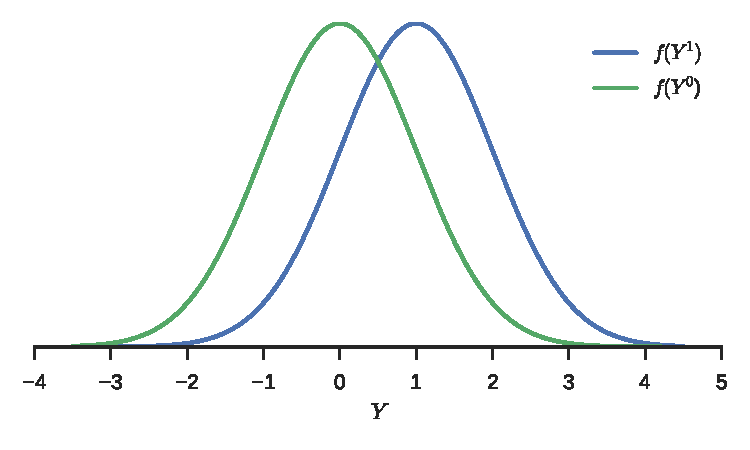
\includegraphics[width=.45\linewidth]{figures/counterfactual_nonidentify_a.pdf}}
\hspace{0.02\textwidth}
\subcaptionbox{Two very different distributions of individual causal effects consistent with the potential outcome distributions. \label{fig:metaphys_b}}
{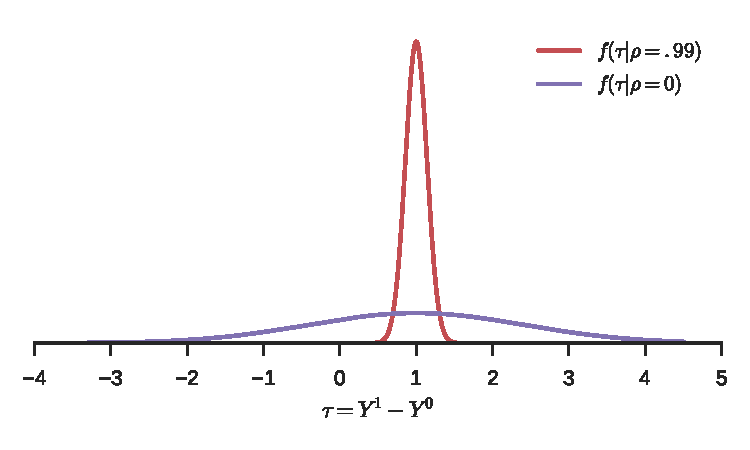
\includegraphics[width=.45\linewidth]{figures/counterfactual_nonidentify_b.pdf}}
\caption{The distribution of individual treatment effects is not identifiable, even from a randomised controlled trial.}
\label{fig:metaphysical_distribution_difference}
\end{figure}

From a (large) randomised controlled trial we can estimate the marginal distributions over the counterfactual variables, see figure \ref{fig:metaphys_a}. These represent the distributions we would expect over the outcome $Y$ if everyone were treated or not treated respectively. However, the distribution over the individual causal effects depends on $\rho$, see figure \ref{fig:metaphys_b}. The key problem is that we can never observe the joint distribution over $\cf{Y}{1}$ and $\cf{Y}{0}$. As a result, $\rho$ and thus the variance of $\tau$ is not identifiable, even from experimental data. \citet{Dawid2000} argues that we should avoid using counterfactuals as they are defined in terms of (metaphysical) individual causal effects. He further points out that the interventional distributions in figure \ref{fig:metaphys_a}, along with a loss function, contain all the information required to decide how to treat a new patient.  

This result is unintuitive. It seems on the face of it that the distribution of individual causal effects is relevant to our decision making. If $\rho = 1$ then almost everyone benefits slightly from the treatment whilst if $\rho=0$, there is a wide range, with some people benefiting a lot and others suffering significant harm. This confusion can be resolved by thinking about personalised rather than individual causal effects. It is entirely possible that potentially observable characteristics (such as gender, age, genetics, etc) affect how people will respond to the treatment. We can partition people into sub-populations on the basis of these characteristics and measure different \emph{personalised} causal effects for each group. The variance of the potential outcome distributions $f(\cf{Y}{1})$ and $f(\cf{Y}{0})$ provides bounds on how much can be gained from further personalisation. The metaphysical nature of individual causal effects only arises when we are at the point where the only remaining variation is due to inherent randomness (or variables that we could not even in principle measure). 



